
%%%%% This is comments

\documentclass[a4paper,10pt]{article}  %% article format
\usepackage{graphicx,amssymb,amsmath,amsthm,textcomp} %%  different package for mathsymbol
\usepackage{mathrsfs}
\usepackage{microtype}
\usepackage[lined,boxed,commentsnumbered,ruled,vlined,noend,
linesnumbered,boxed]{algorithm2e}  %% package for writing algorithm
\usepackage{subcaption}
\usepackage{authblk} % package for author and institute

%%% more packages 
\usepackage{wrapfig}
\usepackage{IEEEtrantools}
\usepackage{color}

\graphicspath{/Users/souravpati/Documents/paper/}


\bibliographystyle{plain} %% this is for bibliography style


\title{ Summer Research Report: A Variant of Covering Problem }  %%% title of the paper %% think about it
% \titlerunning{PTAS for dominating set of homothetic convex objects via local 
% search} 
%\titlerunning{} 

%% Author names to be sorted according to  the last names

\author[1] {Adit Kumar Parida} 
\author[1]{Sourav Pati}

\affil[1]{National Institute of Technology Silchar, India\\
	
	
	\texttt{\{souravpati, aditparida\}@student.nits.ac.in}}





\makeatletter
\@addtoreset{footnote}{page}
\makeatother
\renewcommand{\thefootnote}{\ifcase\value{footnote}\or(*)\or
	(**)\or(***)\or(****)\or(\#)\or(\#\#)\or(\#\#\#)\or(\#\#\#\#)\or($\infty$)\fi}


%%% Following are some command defined for using different color


\newcommand{\red}{\textcolor{red}}
\newcommand{\blue}{\textcolor{blue}}
\newcommand{\green}{\textcolor{Green}}
\newcommand{\teal}{\textcolor{Teal}}
\newcommand{\magenta}{\textcolor{magenta}}
\newcommand{\cyan}{\textcolor{cyan}}
\newcommand{\navy}{\textcolor{Navy}}
\newcommand{\gray}{\textcolor{Gray}}
\newcommand{\darkmagenta}{\textcolor{DarkMagenta}}
\newcommand{\mediumpurple}{\textcolor{MediumPurple}}
\newcommand{\gold}{\textcolor{Gold}}
\newcommand{\darkorange}{\textcolor{DarkOrange}}




\newcommand{\IR}{\mathbb{R}}    %% for R^2




\usepackage{chngcntr}
\counterwithout{paragraph}{subsubsection}
\renewcommand{\theparagraph}{}



%% some more definitions which we may use later


\newtheorem{theorem}{Theorem}
\newtheorem{lemma}{Lemma}
\newtheorem{prop}{Proposition}
\newtheorem{obsv}{Observation}
\newtheorem{result}{Result}
\newtheorem{definition}{Definition}
\newtheorem{observation}{Observation}
\newtheorem{cor}{Corollary}
\newtheorem{remark}{Remark}
\newtheorem{fact}{Fact}
\newtheorem{property}{Property}
\newtheorem{invariant}{Invariant}

\newtheorem{claim}{Claim}

\everymath{\displaystyle}

\setlength{\parskip}{1.2mm}
\setlength{\parindent}{0pt}
\setlength{\textheight}{9.3in}
\setlength{\textwidth}{6.3in}
\renewcommand{\baselinestretch}{1.15}
\setlength{\oddsidemargin}{-0.1in}
\setlength{\topmargin}{-0.1in}


%%% Here begins the document  and will and when \end{document} is reached for the first time
\begin{document}
	
		\maketitle
		\begin{center}
					\large \textbf{Advisor :} Minati De
					
					
					\large\textbf{University :} Indian Institute Of Science, Bengaluru
		\end{center}

	
	
	\cleardoublepage
	\tableofcontents
	\cleardoublepage
	  %% for creating title appropriately
	\section{Abstract}
		
		\large In this summer research report, we discuss about the problems we studied and analyzed for our research work. We studied 4-factor and 3-factor algorithms for solution of geometric minimum dominating set problem. We obtain a 4-factor algorithm by splitting the plane into hexagonal grid which takes O($n^{7d}$). In 3 - factor algorithm it takes O$(n^{18d})$ time to obtain solution. A simplified version of the 3D problem is also considered and provided with a $8 - factor$ algorithm.
	
	\cleardoublepage
	
	%\newpage
	
	\section{Introduction}
	%\vspace{-0.05in}
	\subsection{Problems Definition}
	
	\large Given a set of points $p_i \in {\cal P}$ with demand $d$ each, there exist a set $S \subseteq {\cal P}$ such that unit disks placed on the points in $S$ will cover all the points in ${\cal P}  \backslash  S$ with all its demand satisfied. To satisfy one point's demand we need to cover it with at least d many disks. 
	
	\subsection{Motivation}
	
	\large Our motivation comes from real world application in the usage of wireless sensor network where there are towers at certain points in the 2-Dimensional Euclidean space to satisfy the demands of users placed in regions within the same Euclidean space. Here a new problem may arise when the demand of  each user may not be satisfied with a single tower and thereby require multiple towers to cover their demands. This real world problem can be represented mathematically as a multi cover problem or a piercing set problem where the points associated with the 2D space represent each user with a demand $d$, satisfied by multiple towers surrounding it.
	
	
	\setlength{\parskip}{5.2mm}
	\setlength{\parindent}{0pt}
	\setlength{\textheight}{9.3in}
	\setlength{\textwidth}{6.3in}
	\renewcommand{\baselinestretch}{1.15}
	\setlength{\oddsidemargin}{-0.1in}
	\setlength{\topmargin}{-0.1in}
	
	
	\section{Survey}
	We analysed  PTAS for Weighted Set Cover on Unit Squares by Erlebach and Leeuwen \cite{ErlebachL10} where a PTAS for Geometric Set Cover on any set of axis-parallel unit squares is proposed. A optimal solution for a set of points on a horizontal strip of height $k$ was found in $n^O$$^($$^k$$^)$ with the use of sweep line algorithm. Combining this with the well-known shifting technique yields the PTAS.
	
	\par A PTAS for the Weighted Unit Disk Cover Problem by  Li and Jin\cite{LiJ15}, a paper on weighted disk cover problem provides $(1+\epsilon)$ - factor algorithm. Overall time complexity of the dynamic program is O($n^2$${^K}^{2}$$^+$$^1$) = $n^{O(1/\epsilon^{4})}$.
	
	\par Next, we focused on dominating set problem using local search to apply the multi cover concept for unweighted points. A research work done by Gibson and Pirwani in Approximation Algorithms for Dominating Set in Disk Graphs\cite{matt3320}, which uses local search to find PTAS for the solution of problem. We start with a feasible solution first. Consider $D$ is a set of disk from which we need to find a dominating set. $B \subseteq D$ is $b$-locally optimal if one cannot obtain a smaller dominating set by removing a subset $X \subseteq B$ of size at most $b$ from $B$ and replacing that with a subset of size at most $|X|-1$ from $D\backslash B$. Local search gives a $b$-locally optimal set of disks for $b = c/\epsilon^2$ where $c > 0$ is a large constant. Local search start with arbitrary solution set $B$ and continues to do local improvements. It stops when no further local improvements are possible. 
	
	If a disk in $b$ is properly contained in another disk of $D \backslash B$, then we replace it by the larger disk from $D\backslash B$. Our replacement step ensures that there is no disk in $B$ which is properly contained in some other disk in $D$.
	
	\textbf{Locality Condition:} Let $R$ be the disks obtained from optimal solution and $B$ be the disks obtained from the local algorithm. Then there exists a planar graph with vertex set $R \cup B$, such that for every $d \in D$, there is a disk $u$ from amongst the red dominators of $d$ and a disk $v$ among the blue dominators of d such that ${u, v}$ is an edge in the graph. \cite{matt3320}
	
	Above Condition was proved by the use of weighted voronoi diagram. Meticulous observation will prove that the diagram made by $R \cup B$ is actually star shaped and planner. Using the theorem of planarity by G. N. Frederickson, Fast algorithms for shortest paths in planar graphs with
	applications\cite{Frederickson87}, we can use a planner separator to prove that our solution is $1+\epsilon$ factor of optimal solution.

	
	
	
	

	\subsection{Local Search Algorithm}
	
	\textbf{Algorithm:}\cite{DeL16}
	
	\textbf{Input:} A set of $n$ objects ${\cal P}$ in $\mathbb{R}^2$\\
	1. Initialize ${\cal Q}$ to an arbitrary subset of ${\cal P}$ which is a feasible solution\\
	2. while $\exists$ ${\cal X}\subseteq {\cal Q}$ of size at most $b$, and $X_0 \subseteq  {\cal P}$ of size at most ${\cal X}-1$ such that $({\cal Q} \cap {\cal X}) \cup X_0$ is a feasible solution. do\\
	3. set ${\cal Q}\longleftarrow({\cal Q}\backslash{\cal X})\cup X_0$\\
	4. while $\exists$ some object $Q\in {\cal Q}$ such that region $Q \backslash \bigcup _{P(\neq Q)\in {\cal Q}} P$ is completely contained in some object $R \in {\cal P} \backslash {\cal Q}$ do\\
	5 replace $Q$ by $R$ in {\cal Q}\\
	6 Report $Q$\\
	
	In the above case, a solution is feasible only when all the demands of the points are satisfied i.e. at least d many disks cover a point $p_i \in {\cal P}$. The subsets of {\cal Q} is called $b$-locally optimal if it is not possible to obtain another feasible solution by removing a subset {\cal X} from {\cal Q} and replacing it by a subset $X_0$ of smaller size. We continue to update our solution until no such $X_0$ can be replaced. After obtaining the {\cal Q} from the first loop we check whether the object in {\cal Q} are properly contained by any other objects in the set. If they are contained by any other object, we replace it.
	
	The time taken by the first loop is O($n$) and each iteration consumes time in O($n^b$). So total time for completion of first loop will be O($n^{b+1}$). Second loop needs at most O($n^2$) time. Hence running time of the algorithm is O($n^{b+1}$).
	
	\textbf{Analysis:}
	
	In case of geometric minimum dominating set local search is guaranteed to give $(1+\epsilon)$ factor approximation. The proof is based on the graph separator theorem proposed by G. N. Frederickson, Fast algorithms for shortest paths in planar graphs, with applications\cite{Frederickson87}. Above theorem is applicable only to planner graphs. So we will approach our problem by creating the graph by setting the locality condition. If we can prove the graph to be planner then with the help of planarity theorem proposed by Frederickson we can prove that we have $(1+\epsilon)$- approximation algorithm.
	
	Now, we consider an optimal solution is ${\cal OPT}$. the optimal solution, ${\cal OPT}$, must have less or equal number of disks compared to any other solutions obtained from our algorithm. But in every feasible solution set, the demands of points are satisfied. So at least $d$ many disks must cover each point. ${\cal ALG}$ is considered to be our solution set from the algorithm. We can derive our locality condition for multi cover problem from the locality condition stated in geometric minimum dominating set problem\cite{matt3320}.
	
		
	\textbf{Notation:}
		
	Let ${\cal OPT}$ be the optimal solution and {\cal Q} be the solution returned by our local search algorithm. Our algorithm ensures that there is no object $S \in {\cal S}$ $\backslash$ ${\cal Q}$ which completely contains any object of ${\cal Q}$. Similarly, we can assume that no object in ${\cal OPT}$ is completely contained in any object from $S \backslash {\cal OPT}$. Let ${\cal Q}'={\cal Q} \backslash({\cal Q}\cap{\cal OPT})$, ${\cal OPT}'={\cal OPT} \backslash ({\cal Q}\cap {\cal OPT}) $. We show that $|{\cal Q}'| \leq (1 + \epsilon)|{\cal OPT}'|$ which implies that $|{\cal Q}| \leq (1 + \epsilon)|{\cal OPT} |$.
		
	
	\textbf{Locality Condition :}
	
	\begin{lemma}\label{loca}[Locality Condition]
		There exist a graph ${\cal G} = ({\cal ALG},{\cal OPT},{\cal E})$, where there is at least $d$ number of unit disks $u_i$ covering a point $p_i \in P$ from set ${\cal ALG}$ and $d$ number of unit disks $v_i$ from ${\cal OPT}$ such that there are $d$ many edges between ($u_i,v_i$).
	\end{lemma}
	
	
	
	\textbf{Analysis of Locality Condition:}
	
	We will consider an edge between $u \in {\cal ALG}$ and $v \in {\cal OPT}$, if they cover a same point $p \in {\cal P}$. In our problem, each point has $d$ demand. Hence there are at least $d$ many disks covering each point from each set ${\cal ALG}$ and ${\cal OPT}$. Without loss of generality, we can assume that ${\cal ALG}$ and ${\cal OPT}$ are disjoint sets. ${\cal ALG} \cap {\cal OPT}$ = $\phi$.  So we can derive the conclusion that for a point $p_i$, $d$ disks from {\cal ALG} and $d$ disks from ${\cal OPT}$ are distinct disks. Consider a disk which covers $p_i$ and belongs to ${\cal ALG}$. It will have an edge with disks from ${\cal OPT}$ covering the same point $p_i$. So for $d$ disks in ${\cal OPT}$ we will have total $d$ number of edges to ${\cal OPT}$.
	
	
	
		\begin{lemma}\label{lem_loc_cov}[Locality Condition for Set Cover]
			There exists a planar graph $ {\cal G}=({\cal Q}'\cup {\cal OPT}', {\cal E})$ 
			such that for all 
			$p\in {\cal P}'$ there exists an edge $(U,V)\in {\cal E}$ where both $U$ and 
			$V$ covers
			${\cal P}'$, and  $U\in {\cal Q}'$ and $V\in {\cal OPT}'$.  
		\end{lemma}
		
		
		
		\begin{align}\label{eq0}
		|{\cal Q}_i'|\leq |{\cal OPT}_i'|+|N({\cal V}_i)|,
		\end{align}%\vspace{-0.1in}
		
		{
			\begin{IEEEeqnarray*}{rcl's}
				|{\cal Q}'|
				& \leq & |{\cal X}|+ \sum\limits_{i}|{\cal Q}_i'| & (Each element of ${\cal 
					Q}'$ 
				either belongs to 
				${\cal Q}_i'$ or ${\cal X}$)\\
				& \leq & |{\cal X}| + \sum\limits_{i}|{\cal OPT}_i'|+ \sum\limits_{i}|N({\cal 
					V}_i)| & (Follows from 
				Equation~\ref{eq0}) \\
				& \leq & |{\cal OPT}'|  + |{\cal X}| +  \sum\limits_{i}|N({\cal V}_i)| & 
				(${\cal 
					OPT}_i'$ are disjoint subset 
				of ${\cal OPT}'$)\\
				& \leq & |{\cal OPT}'| + \frac{c'_1(|{\cal Q}'|+|{\cal OPT}'|}{\sqrt{b}} & 
				($|N({\cal V}_i)|\leq c_3 \sqrt{r}$ and $|{\cal X}|\leq c_1 |({\cal Q}'+ {\cal OPT}')|/ \sqrt{r}$ )\\
				|{\cal Q}'| & \leq & \frac{1+c'_1/\sqrt{b}}{1-c'_1/\sqrt{b}}|{\cal OPT}'| & (By 
				rearranging)\\
				|{\cal Q}'| & \leq & (1+\epsilon)|{\cal OPT}'| & ($b$ is large enough constant 
				times 
				$\frac{1}{\epsilon^2}$). 
			\end{IEEEeqnarray*}
		}
			
		
	In the paper, Minimum Dominating Set Problem for Unit Disks Revisited by Carmi et al \cite{CarmiDJNPS15} a 5 - factor approximation algorithm is proposed which runs in O($n$ $log$ $k$) time. ($k$ is size of output). A $4$ factor approximation algorithm is broached by dividing the plane into hexagonal grid instead of rectangular grid. Time complexity of the algorithms is O($n^7$), which can be improved to O($n^6log$ $n$). After using shifting strategy we yield PTAS from Geometric Minimum Dominating Set problem\cite{DeDCN13}. This technique helps us in  our work for multi cover problem.
	
	
	\section{Our Contribution}
	
	 We fixed the demand $d = 2$ for simplification and used the algorithm as discussed in Minimum Dominating Set Problem for Unit Disks Revisited by Paz Carmi et al.\cite{CarmiDJNPS15}. We first obtained a $4$-factor approximation algorithm for demand $d=2$ using hexagonal grid with a time complexity of O($n^{14}$) and then generalized it for a general case of demand $d$ with a time complexity of O($n^{7d}$).
	
	
	\textbf{Simplifying The problem.}
	
	Now, we consider $d = 2$ for the purpose of further simplification. We try to solve the problem with a different approach by dividing the plane $\mathbb{R}^2$ on which the points reside. 
	
	\subsection{4-Factor Approximation Using Hexagonal Grid}
	We first partition a region $\mathbb{R}^2$ containing points in the set ${\cal P}$ into regular hexagonal cells, where the side length of each cell is $\frac{1}{2}$. The length of the diagonal is 1.
	
	\textbf{Observation 1} \textit{Since any pair of points within the hexagonal cell is at most 1 distance apart (length of diagonal is one), an unit disk placed at any point in the cell can cover all the points within that cell(see figure \ref{fig:sfig1})}.
	
	\textbf{Definition} A septa-hexagon is a combination of 7 adjacent cells such that the center cell is surrounded by six similar cells (see Figure \ref{fig:sfig2}).
	
	\begin{figure}
		\begin{subfigure}{.5\textwidth}
			\centering
			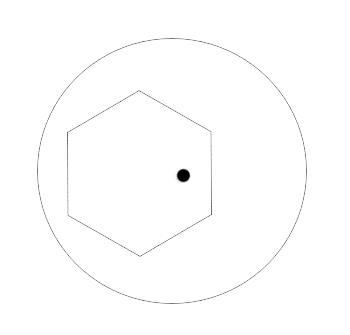
\includegraphics[width=.8\linewidth]{hexa1.png}
			\caption{Unit Radius Disk Covering a Hexagonal Cell}
			\label{fig:sfig1}
		\end{subfigure}%
		\begin{subfigure}{.5\textwidth}
			\centering
			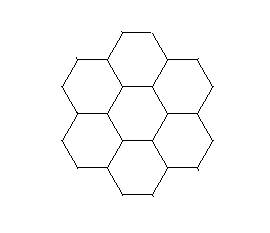
\includegraphics[width=.8\linewidth]{hexa2.png}
			\caption{A Septa-Hexagon}
			\label{fig:sfig2}
		\end{subfigure}
		\caption{Hexagonal Grid}
		\label{fig:fig1}
	\end{figure}
	
	We consider hexagonal grid in $\mathbb{R}^2$ such that no point $p_i \in {\cal P}$ lie on the boundary of the grid. Next we implement a four coloring scheme on it, where each septa-hexagon is assigned a color and no two adjacent septa-hexagon is assigned same color. So if a septa-hexagon is colored $A$ then its adjacent septa-hexagon will be colored $B,C$ $and$ $D$ and each pair of those adjacent septa-hexagon with same color(say $B$) will be opposite to each other.(see figure  \ref{fig:sfig4})
	
	Let us consider the septa-hexagon of a particular color and study its geometry. This leads to the following observation.
	
	\textbf{Observation 2} \textit{Since the septa-hexagon is constituted of regular hexagonal cells of side length 1/2, the minimum distance of two opposite points on the boundary of the septa-hexagon is 2.} 
	
	Now, let the septa-hexagon be  ${\cal T}$ and its two adjacent similar colored septa-hexagon be ${\cal T}'$ and ${\cal T}''$. We can conclude from the a above observation that, if a tower of unit radius is placed at any point in a segment ${\cal T}'$ will never pierce or intersect any point in the segment ${\cal T}''$. Mathematically, if ${\cal T}'$ and ${\cal T}''$ are two closest septa-hexagon with same color then a tower of disk $D$ cannot simultaneously cover a point $p \in {\cal T}' \cap {\cal P} $ and a point $q \in {\cal T}'' \cap {\cal P} $. So, we can consider each colored segment independently i.e. let us take all the segment of color (say $A$). 
	
	\begin{figure}
		\centering
		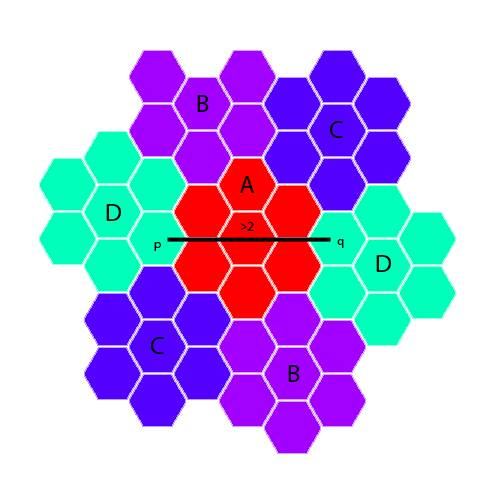
\includegraphics[ width=.6\linewidth] {septa.jpg}
		\caption{4-Coloring Scheme in Hexagonal Grid}
		\label{fig:sfig4}
	\end{figure}
	
	
	\begin{lemma}\label{poly}[Polynomial Time Complexity]
		A solution comprising of towers placed in the region of a particular color(say $A$) of a 4-color scheme septa-hexagon ${\cal ALG_A}$, satisfying demand $d$, can be obtained in a polynomial time of order O($n^{7d}$).
	\end{lemma}
	\begin{proof}
		Consider the septa-hexagon ${\cal T}$ having color (say $A$). We first assume that each of the points has a demand $d=2$. Since each hexagonal cell can be completely covered by the disk of unit radius, we can say that a maximum of 7 disks are necessary to cover a septa-hexagon once. In order to solve this we start by taking all combination of points $i=1,2,3...7$ and return the result that is satisfied by minimum number of disks. This algorithm will return a solution better than optimal solution for a single septa-hexagon and also the time complexity to go through all the combination will be of the order O($n^7$). Similarly, we can say that if each point $p \in {\cal P}$ is associated with demand 2, then we need to cover the entire individual region twice and for that we require a maximum of 14 disks. If we employ a similar strategy  by taking all combination of points $i = 2,3...14$ and return the result that is satisfied by minimum number of disks, we are still able to achieve it in a linear time of O($n^{14}$). This can be generalized further with each point having demand $d$ and still the time complexity will remain polynomial i.e. O($n^{7d}$).
	\end{proof}
	
	Let us consider the result we obtained after solving the region having color $A$ is ${\cal ALG_A}$.  We can observe that $|{\cal ALG_A}|\leq |{\cal OPT}|$ as ${\cal ALG_A}$ covers a partial region of the entire plane in $\mathbb{R}^2$, while ${\cal OPT}$ covers the entire plane.
	
	\begin{lemma}\label{4fac}[4-Factor Approximation]
		$|{\cal ALG}| \leq 4$ $|{\cal OPT}|$, where ${\cal ALG}$ is the solution obtained from the algorithm and ${\cal OPT}$ is the optimal solution such that they cover all the point while satisfying the demand $d$.
	\end{lemma}
	\begin{proof}
		
		From above, we know that $|{\cal ALG_A}| \leq |{\cal OPT}|$. Similarly, $|{\cal ALG_B}|,|{\cal ALG_C}|,|{\cal ALG_D}|\leq |{\cal OPT}|$ as each of the colored elements cover partial region\cite{CarmiDJNPS15}.
		\begin{align*} 
		|{\cal ALG}_A|\leq |{\cal OPT}|,\\ 
		|{\cal ALG}_A|\cup|{\cal ALG}_B|\cup|{\cal ALG}_C|\cup|{\cal ALG}_D|\leq 4|{\cal OPT}|,\\
		|{\cal ALG}|\leq 4|{\cal OPT}|
		\end{align*}%\vspace{-0.1in}
	\end{proof}
	\theoremstyle{theorem}
	\begin{theorem}
		Given a set ${\cal P}$ of $n$ points in $\mathbb{R}^2$ with demand $d$ each, proposed algorithm gives a $8 - $ approximation solution to our problem in time complexity of O($n^{7d}$).
	\end{theorem}
	
	\subsection{3-Factor Approximation Using Rectangular Grid}
	
	Main idea for our problem is taken from the paper\cite{DeDCN13}. In this case, we will partition the plane into horizontal strips of uniform width of $\frac{3}{\sqrt{2}}$. The odd numbered strip will be divided into blocks of length $= \frac{6}{\sqrt{2}}$. In the even numbered strips, it starts with block of length $\frac{3}{\sqrt{2}}$ and continues with $\frac{6}{\sqrt{2}}$ lengths. Then we start coloring the plane blocks using three different colors. Three colors are enough to color them in a way that two blocks with same color are not adjacent. 
	
	\begin{figure}
		\centering
		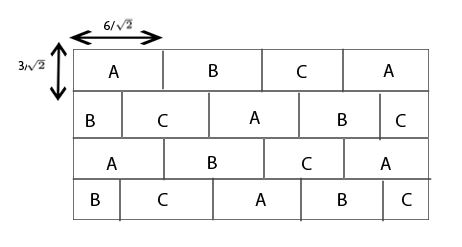
\includegraphics[ width=.6\linewidth] {square.jpg}
		\caption{3-Coloring Scheme In Square Grid}
		\label{fig:sfig5}
	\end{figure}
	
	
	
	Now, we divide each block into smaller blocks of size $\frac{1}{\sqrt{2}}$ of each side.If we calculate, $18$ number of smaller blocks can be accommodated in the larger block of size $\frac{6}{\sqrt{2}} \times  \frac{3}{\sqrt{2}}$. The diagonal of each smaller block will be $1$ unit each. So one disk is enough to cover one smaller block. At most $18$ disks will be required to cover the larger block. Now, we can pick $18$ disks from $n$ disks inside the block to cover it completely. But in our problem each point has a demand $d$. So we have to pick $d$ disks from the smaller blocks to cover the block entirely and satisfy the demands of points inside it. For the larger block it will require at most $18 \times d$ disks to cover the points and satisfy all the demands as well. So the time taken for choosing at most 18d disks will be  O$(n^{18}$$^d)$.
	
	
	
	\begin{lemma}\label{sq}[3-Factor Approximation]
			$|{\cal ALG}| \leq 3$ $|{\cal OPT}|$, where ${\cal ALG}$ is the solution obtained from the algorithm and ${\cal OPT}$ is the optimal solution such that they cover all the point while satisfying the demand $d$.
	\end{lemma}
	
	\begin{proof}
		Consider a block $b_i$. Solution acquired to the block from our algorithm be ${\cal ALG}_i$.
		
		So the solution to block colored $A$ is ${\cal ALG}_A$ and others are ${\cal ALG}_B$ and ${\cal ALG}_C$ respectively. 
		
		Optimal solution is noted by the symbol ${\cal OPT}$.
		\begin{align*} 
		|{\cal ALG}_A|\leq |{\cal OPT}|,\\ 
		|{\cal ALG}_A|\cup|{\cal ALG}_B|\cup|{\cal ALG}_C|\leq 3|{\cal OPT}|,\\
		|{\cal ALG}|\leq 3|{\cal OPT}|
		\end{align*}%\vspace{-0.1in}	
	\end{proof}
	
	\theoremstyle{theorem}
	\begin{theorem}
		Given a set ${\cal P}$ of $n$ points in $\mathbb{R}^2$ with demand $d$ each, proposed algorithm gives a $3 - $approximation solution to our problem in time complexity of O($n^{18d}$).
	\end{theorem}
	
	\subsection{Polynomial Time Approximation Scheme}
		
	Using shifting strategy similar to which used in \cite{DeDCN13}, we can obtain PTAS for our problem. We divide the plane in to squares of size $2k \times 2k$ which can contain ($\lceil 2\sqrt{2}k \rceil$) $^2$ number of cubes of size $\frac{1}{\sqrt{2}} \times \frac{1}{\sqrt{2}}$. So we will need at most ($\lceil 2\sqrt{2}k \rceil$) $^2d$ disks to cover the complete square. So using brute force we can choose these disks in O($n^{{\lceil 2\sqrt{2}k \rceil}^2d}$) time complexity.
	
	\theoremstyle{theorem}
	\begin{theorem}
		Given a set ${\cal P}$ of $n$ points in $\mathbb{R}^2$ and an integer $k \geq 1$, the proposed algorithm delivers a discrete piercing set of the disks centered at all the points of ${\cal P}$ in O($k^2$ $n^{{\lceil 2\sqrt{2}k \rceil}^2d}$) time, whose size is at most ($1 + \frac{1}{k}$) $^2 {\cal OPT}$, where ${\cal OPT}$ is the size of the Optimal solution\cite{DeDCN13}.
	\end{theorem}
	
	\section{Generalizing Problem to 3 Dimension}
	
	Our problem can be generalized to a 3 Dimensional space where instead of unit disks we will consider unit spheres. Each sphere will have demand $d = 1$. We can divide the plane into cubes of size $\frac{4}{\sqrt{3}} \times \frac{4}{\sqrt{3}} \times \frac{4}{\sqrt{3}}$. 
	
	
	
	\theoremstyle{definition}
	\begin{definition}{Disjoint cubes :}
		Two cubes are said to be disjoint or non adjacent if and only if they do not share a face or an edge or a vertex.
	\end{definition}
	
	One cube can be adjacent to maximum 26 number of cubes. The position will be in the middle most cube of the 3 dimensional cubic matrix with $3 \times 3 \times 3$ cubes arranged in a cubic manner. Proposed matrix can be denoted in the $3$- dimensional array notation(matrix[dimension][row][column]).We will denote our matrix by the variable $M[dimension][row][column]$. We will adapt the zero-based indexing system. So $0^{th}$ element will be the first element in our sequence. For an example; $M[0][0][0]$ is the first element in the first row of the first dimension.
	
	Our next step is to color the cubes inside of our matrix. The rule to color the cubes is : no adjacent cubes are given the same color. Following this rule we can color the entire matrix using at least $8$ different colors. 
	
	\subsection{Coloring Scheme}
	
	We can infer from the structure of the matrix $M$ that the middle cube in position $M[1][1][1]$ will be adjacent to every other cube in our matrix. Hence, we can give it a color different to every other cubes. Assume the color is $A$. We can remove the colored cube from our matrix for simplification of further coloring. As no adjacent cube will be given same color, we start looking for disjoint subset of cubes from the remaining matrix an give them a single color. The corner most cubes are disjoint to each other. So the cubes $M[0][0][0], M[0][0][2], M[0][2][0], M[0][2][2], M[2][0][0], M[2][0][2], M[2][2][0], M[2][2][2]$ are given one color, say $B$. The middle cube of the opposite faces can be given one color. So $M[0][1][1] and M[2][1][1]$ is colored with $C$. Similarly we can color $M[1][1][0] and M[1][1][2]$ with $D$ and $M[1][0][1] and M[1][2][1]$ with $E$. We remove them after coloring. Now, 3 disjoint subsets, $\{M[1][0][0], M[1][0][2], M[1][2][0], M[1][2][2]\} , \{ M[0][0][1], M[0][2][1], M[2][0][1],\\ M[2][2][1] \}, \{ M[0][1][0], M[0][1][2], M[2][1][0], M[2][1][0] \}$  remain which can be given color $ F, G, H$ respectively.
	
	Consider our algorithm(discussed later) provides solution for each of the colored cubes. Let us consider our algorithm returns
	${\cal ALG}_A, {\cal ALG}_B, {\cal ALG}_C, {\cal ALG}_D, {\cal ALG}_E, {\cal ALG}_F, {\cal ALG}_G,\\ {\cal ALG}_H$ as our solution set for each colored group. Optimal solution for the problem is considered as ${\cal OPT}$.\
	
	
	\theoremstyle{observation}
	\begin{observation}{}
		Consider two cubes, ${\cal C}_i$ and ${\cal C}_j$, are of same color, then a single sphere can not contain a point from the space covered by ${\cal C}_i$ and ${\cal C}_j$, because the distance between the two points is more than 2.
	\end{observation}
	
		
	\subsection{Algorithm}
	
	The number of sphere required to completely cover a cube of size $\frac{1}{\sqrt{3}} \times \frac{1}{\sqrt{3}} \times \frac{1}{\sqrt{3}}$ is $1$. As the diagonal of the cube is $1$, we can cover the cube in just one sphere. Our larger cube of size
	 $\frac{4}{\sqrt{3}} \times \frac{4}{\sqrt{3}} \times \frac{4}{\sqrt{3}}$ can contain total of $64$ numbers of smaller cubes. So we will need at least 64 number of spheres to completely contain a larger cube. We check all combination of 64 cubes to find our solution which can be carried out in O($n^{64}$) time complexity. 
	 
	 \begin{lemma}\label{cube}[8-Factor Approximation]
	 	$|{\cal ALG}| \leq 8$ $|{\cal OPT}|$, where ${\cal ALG}$ is the solution obtained from the algorithm and ${\cal OPT}$ is the optimal solution such that they cover all the points.
	 \end{lemma}
	 \begin{proof}
	 	Consider a block $b_i$. Solution acquired to the block from our algorithm be ${\cal ALG}_i$.
	 	
	 	Optimal solution be ${\cal OPT}$. Now: \\
	 	\begin{align*} 
	 	|{\cal ALG}_A|\leq |{\cal OPT}|,\\ 
	 	|{\cal ALG}_A|\cup|{\cal ALG}_B|\cup|{\cal ALG}_C| \cup {\cal ALG}_D|\cup|{\cal ALG}_E|\cup|{\cal ALG}_F|\cup{\cal ALG}_G|\cup|{\cal ALG}_H|\leq 8|{\cal OPT}|,\\
	 	|{\cal ALG}|\leq 8|{\cal OPT}|
	 	\end{align*}%\vspace{-0.1in}	
	 \end{proof}
	 \theoremstyle{theorem}
	 \begin{theorem}
	 	Given a set ${\cal P}$ of $n$ points in $\mathbb{R}^3$ using the coloring scheme and applying our algorithm gives us $\cal{ALG} \leq$ $8$  $\cal{OPT}$, where $\cal {ALG}$ is the solution returned to us by our algorithm and $\cal{OPT}$ is the optimal solution in O($n^{64}$) time complexity. 
	 \end{theorem}
	 
		
	\section{Future Scope}
	Further work is possible by considering multi cover problems with variable demands. Here each point can be associated with some demand other than a fixed demand $d$. Also, study related to the multi cover or piercing set problem where there is a fixed demand d, but each point is associated with variable weights. In this case, we can can use a similar strategy as discussed in PTAS for Weighted Set Cover on Unit Squares by Thomas Erlebach and Erik Jan van Leeuwen \cite{ErlebachL10} and A PTAS for the Weighted Unit Disk Cover Problem by Jian Li and Yifei Jin\cite{LiJ15}, by dividing the plane into a small region of $k \times k$ squares and use it to obtain a near ${\cal OPT}$ or ${\cal OPT}$ solution. Then we can employ the concept of shifting strategy to solve it further for a good Approximation Algorithm.
	In the case of 3 Dimensional problem we can give uniform demand $d \geq 2$ which can be further improved to more complex problem such as giving variable demand to each points in 3D space.
	
	
	
	\section{Conclusion}
	
	We have a solution of $4 -$ approximation algorithm for the problem of uniform multi set cover problem which can be solve in O($n^{7d}$) time complexity. Algorithm can be improved to 3 - approximation which can be solved in O($n^{18d}$) time complexity. Then, we obtained PTAS by using shifting strategy. We considered a similar problem in $3 - $ dimensional space and calculated a $8 -$ factor approximation algorithm which requires O($n^{64}$) time complexity. 
	
	%% This is for references
	\bibliographystyle{abbrv}
	\bibliography{references}
	
	
	
	
	
	
\end{document} %% End of template


%%%%% This is comments

